\documentclass[
    12pt,
    openright,
    oneside,
    a4paper,
    english,
    brazil
]{abntex2}

% --- Pacotes Fundamentais ---
\usepackage[utf8]{inputenc}
\usepackage[T1]{fontenc}
\usepackage{lmodern}
\usepackage{microtype}

% --- Matemática e Unidades ---
\usepackage{amsmath}
\usepackage{amsfonts}
\usepackage{amssymb}
% --- Compatibilidade e Definição de Unidades (SI) ---
\makeatletter
\providecommand{\SI}[2]{#1\,#2}
\providecommand{\num}[1]{#1}
\providecommand{\si}[1]{#1}
\providecommand{\qty}[2]{#1\,#2}
\providecommand{\kilo}{\text{k}}
\providecommand{\milli}{\text{m}}
\providecommand{\hertz}{\text{Hz}}
\providecommand{\percent}{\%}
\providecommand{\meter}{\text{m}}
\providecommand{\second}{\text{s}}
\providecommand{\squared}{\textsuperscript{2}}
\providecommand{\per}{/}
\providecommand{\degree}{\ensuremath{^\circ}}
\providecommand{\horsepower}{\text{HP}}
\providecommand{\watt}{\text{W}}
\providecommand{\rpm}{\text{rpm}}
\makeatother

% --- Elementos Visuais e Tabelas ---
\usepackage{graphicx}
\usepackage{booktabs}
\usepackage{multirow}
\usepackage{float}
\usepackage{subcaption}

% --- Citações Padrão ABNT ---
\usepackage[alf,abnt-emphasize=bf,abnt-etal-list=0]{abntex2cite}

% --- Caminho para Imagens ---
\graphicspath{{../results/figures/}}

% --- Informações Institucionais e Metadados ---
\instituicao{Universidade Federal de São João del-Rei \par Curso de Engenharia Mecatrônica}
\autor{Jaime Malafaia de Arêdes Junior}
\titulo{Desenvolvimento de Modelo Preditivo Baseado em Inteligência Artificial para Classificação de Falhas em Rolamentos de Rodeiros Ferroviários}
\orientador[Orientadora:]{Profa. Mariana Geny Moreira Vale Cardoso}
\local{São João del-Rei -- MG}
\data{2026}
\tipotrabalho{Trabalho de Conclusão de Curso (Graduação)}
\preambulo{Trabalho de Conclusão de Curso apresentado à Coordenadoria do Curso de Engenharia Mecatrônica da Universidade Federal de São João del-Rei como requisito parcial para obtenção do título de Bacharel em Engenharia Mecatrônica.}

% --- Configurações de Aparência do PDF ---
\hypersetup{
    colorlinks=true,
    linkcolor=blue,
    citecolor=blue,
    urlcolor=blue,
    bookmarksdepth=4
}

\begin{document}

\selectlanguage{brazil}
\frenchspacing

% --- Elementos Pré-Textuais ---
\imprimircapa
\imprimirfolhaderosto*

\begin{resumo}
Os rolamentos dos rodeiros ferroviários (\textit{axlebox bearings}) operam sob condições dinâmicas severas de carregamento e vibração, constituindo componentes críticos para a segurança e a regularidade do transporte ferroviário de cargas e passageiros. Falhas mecânicas não detectadas nesses elementos podem evoluir para o travamento de eixos e descolamentos estruturais, culminando em descarrilamentos com elevados custos operacionais e riscos à vida humana. Nesse contexto, a manutenção baseada na condição (\textit{Condition-Based Maintenance} -- CBM), fundamentada na análise de vibrações e no Aprendizado de Máquina (\textit{Machine Learning}), surge como uma alternativa preditiva superior às inspeções periódicas preventivas e aos detectores térmicos de via (\textit{hotbox detectors}), os quais identificam anomalias apenas em estágios terminais de degradação. Este trabalho apresenta o desenvolvimento de um \textit{framework} preditivo para diagnóstico e classificação multiclasse de defeitos em rolamentos mecânicos com base no banco de dados experimental de referência da \textit{Case Western Reserve University} (CWRU). O pipeline metodológico compreende a segmentação de sinais de aceleração adquiridos a \SI{12}{\kilo\hertz} em janelas discretas de \num{2048} pontos com preservação de linhagem temporal (\textit{data lineage}), a extração de atributos estocásticos no domínio do tempo (RMS, Curtose, Fator de Crista, Desvio Padrão, Assimetria, Pico a Pico, Fator de Forma e Fator de Impulso) e atributos espectrais baseados na Transformada Rápida de Fourier (FFT com janela de Hanning) e na Análise de Envelope via Transformada de Hilbert, monitorando as frequências características de defeito (BPFO, BPFI, BSF e FTF). Para a modelagem supervisionada, avaliaram-se os algoritmos \textit{Random Forest} e \textit{Support Vector Machines} (SVM com \textit{kernel} RBF e padronização \textit{StandardScaler}). Para evitar vazamento temporal de dados (\textit{data leakage}), empregou-se divisão estratificada por arquivo de ensaio (70/30) e validação cruzada estratificada agrupada (\textit{Stratified Group K-Fold}, $k=4$). Ambos os classificadores alcançaram acurácias superiores a \SI{99}{\percent} no conjunto de teste independente (RF com \SI{99,32}{\percent} e SVM com \SI{99,10}{\percent}). Em nível de ensaio físico completo, a agregação por votação majoritária (\textit{file-level majority voting}) atingiu \SI{100,00}{\percent} de acerto em todos os mancais avaliados, evidenciando a robustez da abordagem para aplicação em sistemas mecatrônicos de monitoramento ferroviário.

\vspace{\onelineskip}
\noindent
\textbf{Palavras-chave:} Manutenção Preditiva. Rolamentos Ferroviários. Processamento de Sinais. Machine Learning. CWRU Dataset.
\end{resumo}

\begin{resumo}[Abstract]
\begin{otherlanguage*}{english}
Railway axlebox bearings operate under severe dynamic loads, impacts, and temperature fluctuations, representing critical components for operational safety and reliability in rail transportation. Undetected mechanical defects in these bearings may progress to axle seizure, wheel derailment, severe financial losses, and hazardous accidents. In this context, Condition-Based Maintenance (CBM) leveraging vibration analysis and Machine Learning algorithms provides an advanced predictive alternative to conventional time-based maintenance and wayside infrared hotbox detectors, which only detect anomalies in terminal failure stages. This work develops an end-to-end computational framework for multi-class fault classification in rolling element bearings using the benchmark dataset from Case Western Reserve University (CWRU). The methodology encompasses signal segmentation into discrete \num{2048}-sample windows with temporal data lineage tracking, followed by feature extraction in both time domain (RMS, Kurtosis, Crest Factor, Standard Deviation, Skewness, Peak-to-Peak, Shape Factor, and Impulse Factor) and frequency domain (Fast Fourier Transform with Hanning windowing and Hilbert envelope spectrum analysis focused on characteristic fault frequencies: BPFO, BPFI, BSF, and FTF). Supervised classification models, specifically Random Forest and Support Vector Machines (SVM with RBF kernel and StandardScaler), were trained and validated. To strictly prevent temporal data leakage, an independent 70/30 train/test split at the file/experiment level and a 4-fold Stratified Group Cross-Validation were implemented. Both classifiers achieved generalization accuracies exceeding \SI{99}{\percent} on the test set (\SI{99.32}{\percent} for Random Forest and \SI{99.10}{\percent} for SVM). Furthermore, an experiment-level majority voting scheme achieved \SI{100.00}{\percent} diagnostic accuracy across all tested bearings, demonstrating the effectiveness and readiness of the proposed methodology for integration into intelligent mechatronic condition monitoring systems.

\vspace{\onelineskip}
\noindent
\textbf{Keywords:} Predictive Maintenance. Railway Bearings. Signal Processing. Machine Learning. CWRU Dataset.
\end{otherlanguage*}
\end{resumo}


\pdfbookmark[0]{\listfigurename}{lof}
\listoffigures*
\cleardoublepage

\pdfbookmark[0]{\listtablename}{lot}
\listoftables*
\cleardoublepage

\pdfbookmark[0]{\contentsname}{toc}
\tableofcontents*
\cleardoublepage

% --- Elementos Textuais ---
\textual

\chapter{Introdução}
\label{cap:introducao}

\section{Contextualização e Definição do Problema}
\label{sec:contextualizacao}

O modal ferroviário desempenha um papel estratégico na infraestrutura logística global, destacando-se pela elevada eficiência energética e capacidade de transporte de grandes volumes de cargas e passageiros em longas distâncias. No cenário industrial contemporâneo, a confiabilidade operacional e a segurança do material rodante constituem requisitos primordiais para a competitividade e sustentabilidade desse setor \cite{smith2015rolling}.

Dentre os subsistemas mecânicos críticos de vagões e locomotivas, os rodeiros ferroviários (\textit{wheelsets}) são responsáveis diretos pela sustentação da carga, guiamento dinâmico na via permanente e transmissão dos esforços de tração e frenagem. A interface rotativa entre os eixos dos rodeiros e as estruturas dos truques é viabilizada pelas caixas de mancal (\textit{axleboxes}), no interior das quais operam rolamentos de elementos rolantes submetidos a severas solicitações operacionais \cite{randall2011rolling}. Tais componentes estão continuamente expostos a cargas radiais e axiais combinadas, oscilações térmicas, vibrações de alta frequência oriundas da interação roda-trilho e choques mecânicos decorrentes de irregularidades geométricas da via e juntas de dilatação.

Sob esse regime severo de serviço, os rolamentos estão sujeitos a mecanismos progressivos de degradação estrutural, com destaque para a fadiga por contato de rolamento (\textit{Rolling Contact Fatigue} -- RCF), desgaste abrasivo, corrosão por atrito e trincas de subsuperfície. Uma vez deflagrado um defeito pontual em componentes internos -- tais como pistas interna e externa ou nos próprios elementos rolantes --, o impacto mecânico repetitivo durante a passagem das esferas ou rolos acelera a deterioração local, provocando destacamentos superficiais (\textit{spalling}). Caso a anomalia não seja identificada e contida em seus estágios iniciais, a evolução do dano pode provocar a fragmentação catastrófica do componente, culminando no travamento do eixo em plena via e, no limite, no descarrilamento da composição ferroviária, evento de severidade crítica associado a elevados prejuízos financeiros e risco iminente à vida humana.

\section{Justificativa}
\label{sec:justificativa}

Historicamente, o setor ferroviário tem empregado estratégias de manutenção preventiva baseadas em tempo ou quilometragem acumulada para a gestão de caixas de mancal. Embora reduza a incidência de falhas em serviço, essa abordagem rígida apresenta limitações operacionais expressivas: acarreta a substituição prematura de componentes que ainda dispõem de vida útil remanescente ou, inversamente, revela-se incapaz de prevenir falhas incipientes aceleradas por condições anômalas de operação antes do intervalo de revisão programado \cite{mobley2002vibration}.

Adicionalmente, as ferrovias modernas utilizam sistemas de monitoramento wayside instalados ao longo da malha, como os detectores óptico-térmicos de caixas quentes (\textit{hotbox detectors} -- HBDs). No entanto, o princípio de atuação dos HBDs reside na detecção da radiação infravermelha emitida quando o mancal atinge patamares térmicos críticos. Sob a ótica da engenharia de manutenção, o aquecimento térmico representa um sintoma terminal de falha mecânica, decorrente do atrito metal-metal generalizado e da degradação irreversível do lubrificante. Quando um alarme de HBD é deflagrado, a janela temporal para intervenção é mínima, demandando paradas emergenciais que interrompem a circulação da malha \cite{smith2015rolling}.

Em contrapartida, a manutenção preditiva baseada na condição (\textit{Condition-Based Maintenance} -- CBM) por meio da análise de vibrações acelerométricas possibilita a identificação de defeitos mecânicos em seus estágios mais embrionários, semanas ou meses antes do surgimento de calor anômalo perceptível \cite{randall2011rolling}. O impacto de um elemento rolante sobre uma microfissura gera pulsos transitórios de alta frequência que se propagam pela estrutura do mancal, permitindo que ferramentas avançadas de Processamento Digital de Sinais (PDS) e modelos de Aprendizado de Máquina (\textit{Machine Learning}) diagnostiquem o tipo e a severidade do dano com precisão quantitativa.

A validação preliminar de algoritmos inteligentes de diagnóstico requer bancos de dados experimentais controlados e reprodutíveis. Nesse contexto, o dataset de referência da \textit{Case Western Reserve University} (CWRU) consagrou-se como o padrão científico mais adotado na literatura internacional para o desenvolvimento e comparação de modelos preditivos \cite{smith2015rolling}. A aplicação desses dados viabiliza a consolidação de uma metodologia robusta que poderá, subsequentemente, ser transferida e adaptada aos sinais monitorados em rodeiros ferroviários reais.

O desenvolvimento deste trabalho insere-se no núcleo interdisciplinar da Engenharia Mecatrônica, sintetizando conceitos de dinâmica de sistemas mecânicos, instrumentação e sensoriamento eletrônico de vibrações, e computação avançada voltada à modelagem preditiva.

\section{Objetivos}
\label{sec:objetivos}

\subsection{Objetivo Geral}

Desenvolver, implementar e validar um \textit{framework} computacional em linguagem Python para processamento digital de sinais de vibração e classificação multiclasse do tipo e severidade de falhas mecânicas em rolamentos, combinando análise estocástica no domínio do tempo, análise espectral no domínio da frequência e algoritmos de Aprendizado de Máquina aplicados ao banco de dados experimental da CWRU.

\subsection{Objetivos Específicos}

Para a consecução do objetivo geral, estabelecem-se as seguintes metas específicas:
\begin{enumerate}
    \item Desenvolver um módulo de ingestão e pré-processamento de séries temporais brutas adquiridas a \SI{12}{\kilo\hertz}, implementando a segmentação em janelas discretas com rastreabilidade de linhagem de dados (\textit{data lineage});
    \item Extrair descritores estatísticos no domínio do tempo (RMS, Curtose, Fator de Crista, Desvio Padrão, Assimetria, Pico a Pico, Fator de Forma e Fator de Impulso) correlacionados à energia e à impulsividade dos impactos mecânicos;
    \item Implementar o processamento no domínio da frequência por meio da Transformada Rápida de Fourier (FFT com janela de Hanning) e da Análise de Envelope via Transformada de Hilbert, quantificando a energia associada às frequências características de defeito (BPFO, BPFI, BSF e FTF);
    \item Implementar e otimizar classificadores supervisionados baseados em \textit{Random Forest} e \textit{Support Vector Machines} (SVM);
    \item Estruturar protocolos de validação cruzada agrupada (\textit{Stratified Group K-Fold}) para garantir a estrita prevenção de vazamento de dados (\textit{data leakage}) entre janelas do mesmo ensaio físico;
    \item Avaliar o desempenho preditivo dos modelos por meio de matrizes de confusão e métricas acadêmicas (Acurácia, Precisão, Sensibilidade e \textit{F1-Score});
    \item Propor e validar uma estratégia de votação majoritária por ensaio (\textit{file-level majority voting}) para a consolidação do diagnóstico em nível de equipamento completo.
\end{enumerate}

\section{Organização do Trabalho}
\label{sec:organizacao}

Esta monografia está estruturada em cinco capítulos:
\begin{itemize}
    \item O \textbf{\autoref{cap:introducao}} contextualiza a relevância do transporte ferroviário, delineia a problemática associada à falha de rolamentos de rodeiros, apresenta a justificativa e formaliza os objetivos;
    \item O \textbf{\autoref{cap:revisao}} estabelece a fundamentação teórica sobre a dinâmica e os modos de falha em rolamentos de esferas, detalha a matemática do processamento digital de sinais nos domínios do tempo e da frequência, e descreve a formulação dos modelos de Aprendizado de Máquina empregados;
    \item O \textbf{\autoref{cap:metodologia}} descreve detalhadamente o ambiente experimental da CWRU, a arquitetura do pipeline computacional desenvolvido em Python, a rotina de segmentação por janelas, os vetores de atributos extraídos e a metodologia de treino e validação cruzada;
    \item O \textbf{\autoref{cap:resultados}} apresenta e discute os resultados obtidos, confrontando o desempenho dos classificadores, analisando a relevância dos atributos físicos para o diagnóstico e detalhando o comportamento das matrizes de confusão e da votação majoritária por ensaio;
    \item O \textbf{\autoref{cap:conclusao}} sintetiza as principais conclusões alcançadas, destaca as contribuições do trabalho e sugere propostas para pesquisas e desdobramentos futuros.
\end{itemize}

\chapter{Fundamentação Teórica}
\label{cap:revisao}

\section{Dinâmica e Modos de Falha em Rolamentos de Elementos Rolantes}
\label{sec:dinamica_rolamentos}

Os rolamentos de elementos rolantes constituem pares cinemáticos de precisão projetados para suportar carregamentos mecânicos elevados, minimizando as perdas por atrito viscoso e de contato entre componentes em movimento relativo \cite{harris2006rolling}. Em rodeiros e caixas de mancal ferroviárias, a integridade mecânica desses elementos governa a confiabilidade de todo o sistema de tração e sustentação do trem.

Estruturalmente, um rolamento radial típico é composto por quatro elementos fundamentais:
\begin{enumerate}
    \item \textbf{Pista interna (\textit{inner race}):} anel montado solidariamente ao eixo rotativo do rodeiro;
    \item \textbf{Pista externa (\textit{outer race}):} anel fixado ao alojamento estacionário da caixa de mancal (\textit{axlebox});
    \item \textbf{Elementos rolantes (esferas ou rolos):} corpos intermediários que transmitem a carga dinâmica entre os anéis através de áreas de contato hertziano reduzidas;
    \item \textbf{Gaiola espaçadora (\textit{cage}):} estrutura responsável por manter o espaçamento angular uniforme entre os elementos rolantes, prevenindo o contato metal-metal mútuo.
\end{enumerate}

\subsection{Cinemática e Frequências Características de Defeito}
\label{subsec:frequencias_falha}

Quando uma descontinuidade mecânica localizada (como um micropitting, trinca ou cavidade gerada por fadiga de contato) surge em um dos componentes do rolamento, a passagem sucessiva dos elementos rolantes sobre essa superfície danificada gera impactos impulsivos repetitivos de curtíssima duração \cite{randall2011rolling}. A periodicidade temporal desses impactos é estritamente vinculada à cinemática geométrica do rolamento e à rotação do eixo.

Considerando um rolamento operando em regime de contato puro (sem escorregamento cinemático), as frequências cinemáticas fundamentais de repetição dos impactos são deduzidas analiticamente a partir dos parâmetros dimensionais ilustrados na \autoref{fig:geometria_rolamento} \cite{harris2006rolling}:
\begin{itemize}
    \item $d$: diâmetro dos elementos rolantes (esferas ou rolos) [\si{\meter} ou \si{in}];
    \item $D$: diâmetro primitivo ou diâmetro de passo (\textit{pitch diameter}) [\si{\meter} ou \si{in}];
    \item $n$: quantidade de elementos rolantes no conjunto;
    \item $\phi$: ângulo de contato da carga em relação ao plano radial [\si{\degree}];
    \item $f_r$: frequência fundamental de rotação do eixo [\si{\hertz}], calculada a partir da velocidade em rotações por minuto ($\text{RPM}$) por:
    \begin{equation}
        f_r = \frac{\text{RPM}}{60}
        \label{eq:frequencia_rotacao}
    \end{equation}
    onde:
    \begin{itemize}
        \item $f_r$ é a frequência de giro do eixo [\si{\hertz}];
        \item $\text{RPM}$ é a velocidade angular do eixo [\si{rpm}].
    \end{itemize}
\end{itemize}

\begin{figure}[htbp]
    \centering
    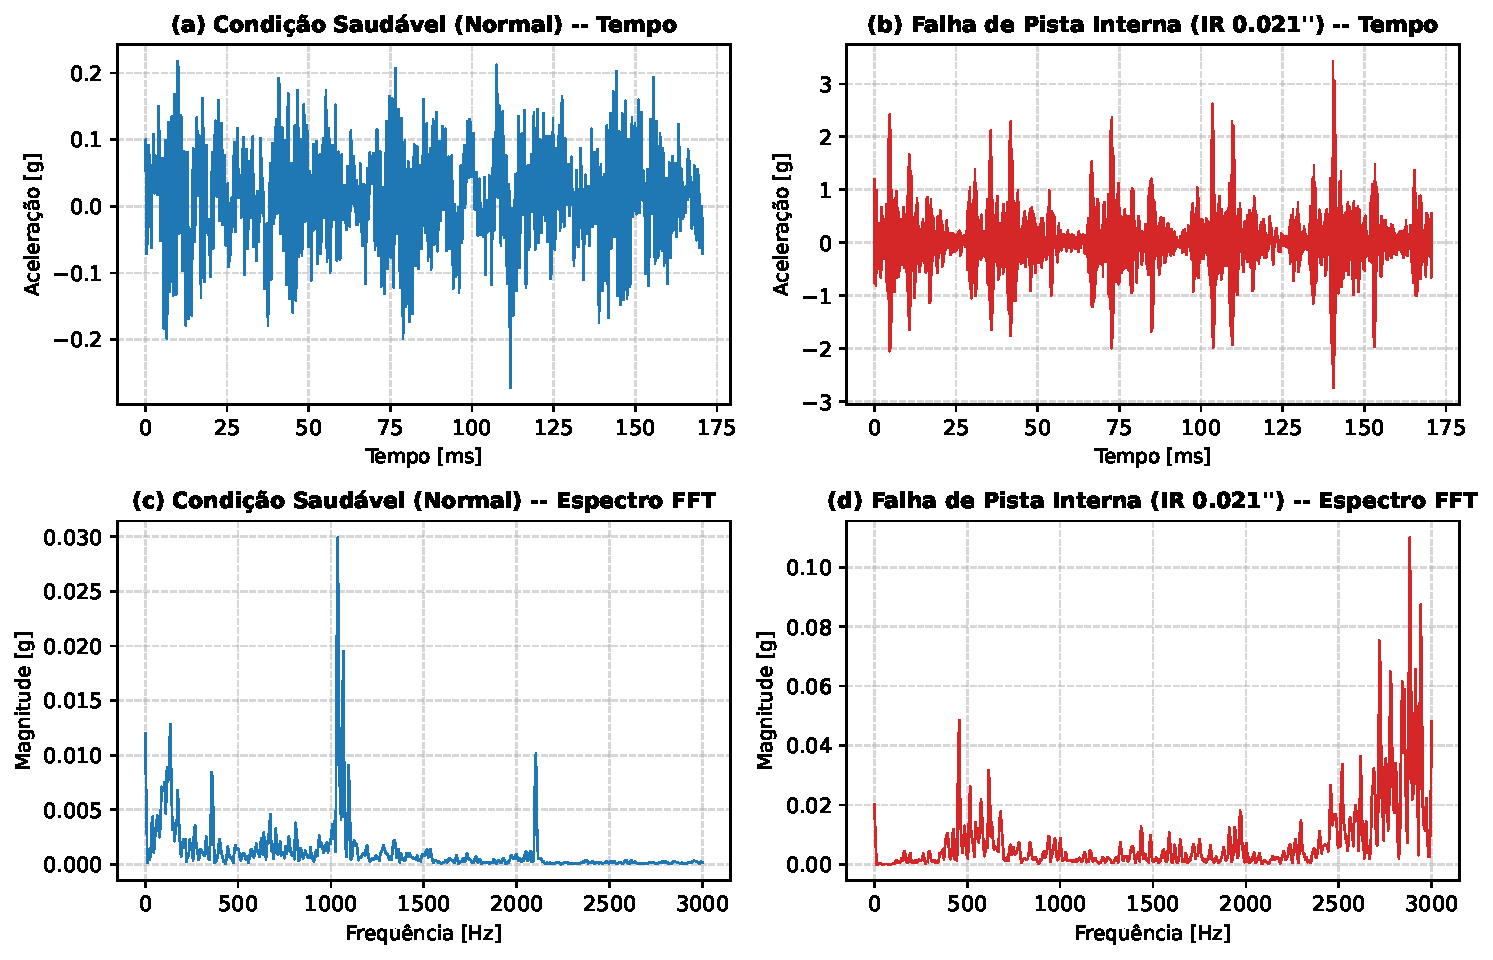
\includegraphics[width=0.55\textwidth]{fig_sinais_tempo_fft.pdf}
    \caption{Representação esquemática dos parâmetros geométricos de um rolamento radial de esferas}
    \label{fig:geometria_rolamento}
    \legend{Fonte: Adaptado de Randall e Antoni (2011).}
\end{figure}

A partir dessas grandezas dimensionais, definem-se quatro frequências características de defeito:

\subsubsection{Frequência de Passagem de Esferas pela Pista Externa (BPFO)}
A frequência BPFO (\textit{Ball Pass Frequency Outer}) corresponde à taxa de repetição dos impactos gerados quando os elementos rolantes transitam sobre um ponto de falha localizado na pista externa estacionária:
\begin{equation}
    \text{BPFO} = \frac{n \cdot f_r}{2} \left( 1 - \frac{d}{D} \cos\phi \right)
    \label{eq:bpfo}
\end{equation}
onde:
\begin{itemize}
    \item $\text{BPFO}$ é a frequência característica de defeito na pista externa [\si{\hertz}];
    \item $n$ é o número de elementos rolantes;
    \item $f_r$ é a rotação do eixo [\si{\hertz}];
    \item $d$ é o diâmetro da esfera [\si{\meter} ou \si{in}];
    \item $D$ é o diâmetro primitivo [\si{\meter} ou \si{in}];
    \item $\phi$ é o ângulo de contato mecânico [\si{\degree}].
\end{itemize}

\subsubsection{Frequência de Passagem de Esferas pela Pista Interna (BPFI)}
A frequência BPFI (\textit{Ball Pass Frequency Inner}) quantifica os impactos decorrentes da passagem dos elementos rolantes sobre um ponto com defeito na pista interna solidária ao eixo rotativo:
\begin{equation}
    \text{BPFI} = \frac{n \cdot f_r}{2} \left( 1 + \frac{d}{D} \cos\phi \right)
    \label{eq:bpfi}
\end{equation}
onde:
\begin{itemize}
    \item $\text{BPFI}$ é a frequência característica de defeito na pista interna [\si{\hertz}], sendo fisicamente superior à $\text{BPFO}$ devido à rotação relativa da pista interna.
\end{itemize}

\subsubsection{Frequência de Giro do Elemento Rolante (BSF)}
A frequência BSF (\textit{Ball Spin Frequency}) representa a rotação própria da esfera em torno do seu próprio centro geométrico. Cada revolução completa da esfera com defeito superficial gera dois impactos sucessivos (um contra a pista interna e outro contra a pista externa):
\begin{equation}
    \text{BSF} = \frac{D \cdot f_r}{2d} \left[ 1 - \left(\frac{d}{D}\cos\phi\right)^2 \right]
    \label{eq:bsf}
\end{equation}
onde:
\begin{itemize}
    \item $\text{BSF}$ é a frequência angular de giro da esfera [\si{\hertz}].
\end{itemize}

\subsubsection{Frequência Fundamental da Gaiola (FTF)}
A frequência FTF (\textit{Fundamental Train Frequency}) expressa a velocidade angular de rotação do conjunto da gaiola que aloja os elementos rolantes em relação ao anel externo estacionário:
\begin{equation}
    \text{FTF} = \frac{f_r}{2} \left( 1 - \frac{d}{D}\cos\phi \right)
    \label{eq:ftf}
\end{equation}
onde:
\begin{itemize}
    \item $\text{FTF}$ é a frequência de revolução do trem de esferas/gaiola [\si{\hertz}].
\end{itemize}

Em rolamentos radiais puros, o ângulo de contato é nulo ($\phi = 0^\circ$), simplificando o termo $\cos\phi = 1,0$ nas \autoref{eq:bpfo} a \ref{eq:ftf}.

\subsection{Mecanismos Físicos de Propagação e Modulação de Vibração}
\label{subsec:modulacao_vibracao}

A detecção de falhas em rolamentos baseada em vibrações envolve aspectos dinâmicos sutis:
\begin{enumerate}
    \item \textbf{Resposta Impulsiva e Ressonância Estrutural:} Os impactos pontuais exercidos pelo defeito comportam-se como trens de impulsos de Dirac no domínio do tempo, possuindo um espectro contínuo de banda larga. Esses impactos excitam as frequências naturais de vibração da carcaça do mancal e do sensor acelerométrico (tipicamente localizadas em faixas de alta frequência, entre \SI{2}{\kilo\hertz} e \SI{10}{\kilo\hertz}) \cite{randall2011rolling};
    \item \textbf{Modulação de Amplitude em Falhas de Pista Interna e Esferas:} Quando a falha situa-se na pista interna, a região danificada gira solidariamente ao eixo, adentrando e saindo periodicamente da zona de carga principal do mancal. Em consequência, a amplitude dos pulsos de vibração gerados na frequência $\text{BPFI}$ sofre modulação em amplitude (\textit{Amplitude Modulation} -- AM) na frequência de rotação do eixo ($f_r$). No domínio da frequência, isso se manifesta pelo surgimento de bandas laterais (\textit{sidebands}) espaçadas de $\pm f_r$ em torno da $\text{BPFI}$ e de seus harmônicos \cite{smith2015rolling};
    \item \textbf{Estacionariedade da Zona de Carga na Pista Externa:} Como a pista externa é estacionária em mancais de rodeiros ferroviários, um defeito centrado no fundo da zona de carga sofrerá impactos de intensidade uniforme a cada passagem de esfera, resultando em menor dispersão por modulação comparativamente às falhas de pista interna.
\end{enumerate}

\section{Processamento Digital de Sinais Aplicado à Análise de Vibrações}
\label{sec:processamento_sinais}

O sinal de vibração discretizado $x[n] = x(n T_s)$ corresponde a uma série temporal de $N$ amostras adquirida a uma taxa de amostragem constante $f_s = 1/T_s$. Para viabilizar a classificação supervisionada por algoritmos de Aprendizado de Máquina, o sinal contínuo deve ser convertido em um conjunto compacto de descritores matemáticos informativos nos domínios do tempo e da frequência \cite{oppenheim2010discrete}.

\subsection{Descritores Estatísticos no Domínio do Tempo}
\label{subsec:features_tempo}

As características no domínio do tempo caracterizam as propriedades estocásticas da série temporal, quantificando energia basal, dispersão e a presença de picos transitórios agudos \cite{antoni2006spectral}:

\subsubsection{Valor Eficaz (Root Mean Square -- RMS)}
O valor RMS quantifica a potência média e a energia cinética global contida no sinal de vibração ao longo da janela:
\begin{equation}
    \text{RMS} = \sqrt{\frac{1}{N} \sum_{i=1}^{N} x_i^2}
    \label{eq:rms}
\end{equation}
onde:
\begin{itemize}
    \item $\text{RMS}$ é o valor eficaz do sinal de aceleração [\si{g} ou \si{\meter\per\second\squared}];
    \item $x_i$ é a $i$-ésima amostra de aceleração discretizada;
    \item $N$ é o número total de pontos na janela de análise.
\end{itemize}

\subsubsection{Curtose (Kurtosis)}
A curtose é o quarto momento estatístico normalizado, constituindo uma métrica sensível à impulsividade do sinal. Valores de curtose próximos a 3 indicam distribuição normal (típica de rolamentos sadios com ruído gaussiano), ao passo que impactos periódicos decorrentes de falhas elevam substancialmente o valor da curtose \cite{antoni2006spectral}:
\begin{equation}
    K = \frac{\frac{1}{N} \sum_{i=1}^{N} (x_i - \bar{x})^4}{\left( \frac{1}{N} \sum_{i=1}^{N} (x_i - \bar{x})^2 \right)^2}
    \label{eq:curtose}
\end{equation}
onde:
\begin{itemize}
    \item $K$ é a curtose adimensional (com convenção de referência em $3,0$ para distribuição gaussiana);
    \item $\bar{x}$ é a média aritmética das amostras da janela.
\end{itemize}

\subsubsection{Fator de Crista (Crest Factor)}
O Fator de Crista expressa a razão entre a amplitude de pico absoluta e a energia média eficaz do sinal, indicando a predominância de choques pontuais em relação ao ruído de fundo:
\begin{equation}
    \text{CF} = \frac{\max_{1 \le i \le N} |x_i|}{\text{RMS}}
    \label{eq:fator_crista}
\end{equation}
onde:
\begin{itemize}
    \item $\text{CF}$ é o fator de crista adimensional ($\text{CF} \ge 1,0$).
\end{itemize}

\subsubsection{Desvio Padrão ($\sigma$)}
O desvio padrão mensura a variabilidade da aceleração em torno da média:
\begin{equation}
    \sigma = \sqrt{\frac{1}{N} \sum_{i=1}^{N} (x_i - \bar{x})^2}
    \label{eq:desvio_padrao}
\end{equation}
onde:
\begin{itemize}
    \item $\sigma$ é o desvio padrão da aceleração [\si{g} ou \si{\meter\per\second\squared}].
\end{itemize}

\subsubsection{Assimetria (Skewness)}
O terceiro momento estatístico quantifica a assimetria da distribuição de probabilidade das amplitudes do sinal em relação à média:
\begin{equation}
    S = \frac{\frac{1}{N} \sum_{i=1}^{N} (x_i - \bar{x})^3}{\sigma^3}
    \label{eq:assimetria}
\end{equation}
onde:
\begin{itemize}
    \item $S$ é o coeficiente de assimetria adimensional.
\end{itemize}

\subsubsection{Valor Pico a Pico (Peak-to-Peak)}
Representa a excursão dinâmica máxima da aceleração instantânea na janela:
\begin{equation}
    X_{p-p} = \max_{1 \le i \le N} (x_i) - \min_{1 \le i \le N} (x_i)
    \label{eq:pico_a_pico}
\end{equation}
onde:
\begin{itemize}
    \item $X_{p-p}$ é a amplitude pico a pico [\si{g} ou \si{\meter\per\second\squared}].
\end{itemize}

\subsubsection{Fator de Forma e Fator de Impulso}
O Fator de Forma ($\text{SF}$) e o Fator de Impulso ($\text{IF}$) relacionam o valor RMS e o valor de pico à média retificada absoluta do sinal, respectivamente:
\begin{equation}
    \text{SF} = \frac{\text{RMS}}{\frac{1}{N} \sum_{i=1}^{N} |x_i|}, \quad \text{IF} = \frac{\max_{1 \le i \le N} |x_i|}{\frac{1}{N} \sum_{i=1}^{N} |x_i|}
    \label{eq:fatores_forma_impulso}
\end{equation}

\subsection{Análise no Domínio da Frequência e Análise de Envelope}
\label{subsec:analise_frequencia}

Embora as estatísticas temporais sejam sensíveis à severidade global do dano, elas não discriminam isoladamente qual componente interno do rolamento está avariado. Essa identificação requer a conversão do sinal para o domínio da frequência por meio da Transformada Discreta de Fourier (\textit{Discrete Fourier Transform} -- DFT) \cite{oppenheim2010discrete}:
\begin{equation}
    X[k] = \sum_{n=0}^{N-1} x[n] \cdot e^{-j \frac{2\pi}{N} k n}, \quad k = 0, 1, \dots, N-1
    \label{eq:dft}
\end{equation}
onde:
\begin{itemize}
    \item $X[k]$ são os coeficientes espectrais complexos na frequência $f_k = k \frac{f_s}{N}$;
    \item $j = \sqrt{-1}$ é a unidade imaginária.
\end{itemize}

Computacionalmente, a DFT é executada mediante o algoritmo da Transformada Rápida de Fourier (\textit{Fast Fourier Transform} -- FFT), reduzindo a complexidade de $\mathcal{O}(N^2)$ para $\mathcal{O}(N \log N)$. 

Para atenuar o fenômeno de espalhamento espectral (\textit{spectral leakage}) provocado pelo truncamento abrupto da janela temporal, aplica-se previamente uma função de janelamento suave, sendo a janela de Hanning a mais consagrada na literatura de vibrações:
\begin{equation}
    w[n] = 0,5 - 0,5 \cos\left( \frac{2\pi n}{N-1} \right), \quad n = 0, 1, \dots, N-1
    \label{eq:hanning}
\end{equation}

\subsubsection{Análise de Envelope via Transformada de Hilbert}
Como destacado na \autoref{subsec:modulacao_vibracao}, as repetições de impacto de baixa frequência ($\text{BPFO}, \text{BPFI}, \text{BSF} < \SI{300}{\hertz}$) modulam em amplitude ressonâncias estruturais de alta frequência ($> \SI{2000}{\hertz}$). Em uma FFT direta, a amplitude nessas frequências baixas pode ficar submersa no ruído basal da máquina \cite{randall2011rolling}.

A Análise de Envelope soluciona essa limitação desmodulando o sinal mediante a construção do sinal analítico complexo $z(t)$ via Transformada de Hilbert $\mathcal{H}\{x(t)\}$:
\begin{equation}
    z(t) = x(t) + j \mathcal{H}\{x(t)\} = x(t) + j \left( \frac{1}{\pi} \text{P.V.} \int_{-\infty}^{\infty} \frac{x(\tau)}{t - \tau} d\tau \right)
    \label{eq:hilbert}
\end{equation}
onde $\text{P.V.}$ denota o Valor Principal de Cauchy da integral imprópria.

O envelope de amplitude instantânea $e(t)$ é definido pela magnitude do sinal analítico:
\begin{equation}
    e(t) = |z(t)| = \sqrt{x^2(t) + [\mathcal{H}\{x(t)\}]^2}
    \label{eq:envelope}
\end{equation}

Como o sinal resultante $e(t)$ é estritamente não negativo, ele carrega um offset de corrente contínua (DC) pronunciado. Para evitar a saturação de energia no bin de \SI{0}{\hertz} da FFT, subtrai-se a média do envelope antes do cálculo espectral:
\begin{equation}
    e_{\text{proc}}(t) = e(t) - \frac{1}{N}\sum_{i=1}^{N} e_i
    \label{eq:envelope_sem_dc}
\end{equation}

A FFT aplicada sobre $e_{\text{proc}}(t)$ revela com clareza os picos espectrais coincidentes com as frequências cinemáticas $\text{BPFO}$, $\text{BPFI}$ e $\text{BSF}$.

\section{Aprendizado de Máquina na Classificação de Falhas}
\label{sec:machine_learning}

\subsection{Classificador Random Forest}
\label{subsec:random_forest}

O algoritmo \textit{Random Forest}, proposto por \citeonline{breiman2001random}, é um método de aprendizado por comitê (\textit{ensemble learning}) fundamentado no princípio do empacotamento estatístico (\textit{bagging} -- \textit{Bootstrap Aggregating}) aplicado a árvores de decisão. 

Em vez de treinar uma única árvore profunda propensa ao sobreajuste (\textit{overfitting}), o modelo constrói uma floresta de $B$ árvores de decisão independentes. Para cada árvore $b \in \{1, \dots, B\}$, seleciona-se uma amostra com reposição do conjunto de treino original. Durante a divisão de cada nó da árvore, avalia-se apenas um subconjunto aleatório de $m \approx \sqrt{p}$ atributos entre os $p$ atributos disponíveis, descorrelacionando os estimadores individuais \cite{breiman2001random}.

A decisão em cada nó é governada pela minimização da impureza de Gini:
\begin{equation}
    I_G(t) = 1 - \sum_{k=1}^{C} p_{t, k}^2
    \label{eq:gini}
\end{equation}
onde:
\begin{itemize}
    \item $I_G(t)$ é o índice de impureza do nó $t$;
    \item $p_{t, k}$ é a proporção de amostras da classe $k \in \{1, \dots, C\}$ presentes no nó $t$.
\end{itemize}

A predição final para uma nova janela de sinal $\mathbf{x}$ é obtida por votação majoritária entre todas as árvores da floresta:
\begin{equation}
    \hat{y} = \arg\max_{c \in \{1, \dots, C\}} \sum_{b=1}^{B} I(h_b(\mathbf{x}) = c)
    \label{eq:votacao_rf}
\end{equation}
onde $h_b(\mathbf{x})$ é o voto emitido pela $b$-ésima árvore. 

O modelo fornece adicionalmente a Importância Média de Redução de Impureza (\textit{Mean Decrease in Impurity} -- MDI), quantificando a contribuição relativa de cada atributo para a pureza da classificação.

\subsection{Support Vector Machines (SVM)}
\label{subsec:svm}

A técnica de Máquinas de Vetores de Suporte (\textit{Support Vector Machines} -- SVM), formalizada por \citeonline{cortes1995support}, busca determinar o hiperplano ótimo em um espaço de características multidimensional que maximize a margem de separação entre as classes de dados.

Dado um conjunto de treinamento $\{(\mathbf{x}_i, y_i)\}_{i=1}^{N}$, com $\mathbf{x}_i \in \mathbb{R}^p$ e rótulos $y_i \in \{-1, +1\}$, a formulação primal com margens suaves (\textit{soft margin}) e penalidade de erro $C > 0$ é expressa pelo problema de programação quadrática convexa:
\begin{equation}
    \min_{\mathbf{w}, b, \boldsymbol{\xi}} \frac{1}{2} \|\mathbf{w}\|^2 + C \sum_{i=1}^{N} \xi_i
    \label{eq:svm_primal}
\end{equation}
sujeito às restrições lineares:
\begin{equation}
    y_i (\mathbf{w}^T \phi(\mathbf{x}_i) + b) \ge 1 - \xi_i, \quad \xi_i \ge 0, \quad \forall i = 1, \dots, N
    \label{eq:svm_restricoes}
\end{equation}
onde:
\begin{itemize}
    \item $\mathbf{w}$ é o vetor normal que orienta o hiperplano divisor;
    \item $b$ é o termo de polarização (\textit{bias});
    \item $\xi_i$ são variáveis de folga que toleram amostras dentro da margem ou mal classificadas;
    \item $C$ é a constante de regularização que equilibra a largura da margem e a penalização por violação de fronteira;
    \item $\phi(\cdot)$ é uma transformação não linear que projeta os dados em um espaço de dimensão superior.
\end{itemize}

Mediante a aplicação das condições de Karush-Kuhn-Tucker (KKT) e a formulação dual de Lagrange, a função de decisão depende exclusivamente de produtos escalares computados eficientemente através de uma função de \textit{kernel} $K(\mathbf{x}_i, \mathbf{x}_j) = \phi(\mathbf{x}_i)^T \phi(\mathbf{x}_j)$ (\textit{kernel trick}) \cite{cortes1995support}. Para padrões vibracionais mecânicos não lineares, o \textit{kernel} Gaussiano de Base Radial (\textit{Radial Basis Function} -- RBF) é o mais recomendado:
\begin{equation}
    K(\mathbf{x}_i, \mathbf{x}_j) = \exp\left( -\gamma \|\mathbf{x}_i - \mathbf{x}_j\|^2 \right)
    \label{eq:kernel_rbf}
\end{equation}
onde $\gamma > 0$ governa o raio de influência das amostras de suporte. Para problemas multiclasse ($C > 2$), o SVM utiliza a estratégia de decomposição Um-contra-Um (\textit{One-vs-One} -- OvO).

\subsection{Métricas de Avaliação Multiclasse}
\label{subsec:metricas_avaliacao}

O desempenho dos classificadores em problemas multiclasse é sintetizado pela Matriz de Confusão, cujas linhas representam as classes verdadeiras do rolamento e cujas colunas representam as predições computadas pelo modelo. A partir das contagens de Verdadeiros Positivos ($\text{VP}$), Falsos Positivos ($\text{FP}$), Falsos Negativos ($\text{FN}$) e Verdadeiros Negativos ($\text{VN}$) para cada classe $k$, computam-se as seguintes métricas fundamentais:
\begin{equation}
    \text{Acurácia Global} = \frac{\sum_{k=1}^{C} \text{VP}_k}{\sum_{k=1}^{C} (\text{VP}_k + \text{FP}_k + \text{FN}_k)}
    \label{eq:acuracia}
\end{equation}
\begin{equation}
    \text{Precisão}_k = \frac{\text{VP}_k}{\text{VP}_k + \text{FP}_k}, \quad \text{Sensibilidade}_k (\textit{Recall}) = \frac{\text{VP}_k}{\text{VP}_k + \text{FN}_k}
    \label{eq:precisao_recall}
\end{equation}
\begin{equation}
    \text{F1-Score}_k = 2 \cdot \frac{\text{Precisão}_k \cdot \text{Sensibilidade}_k}{\text{Precisão}_k + \text{Sensibilidade}_k}
    \label{eq:f1_score}
\end{equation}

A média macro (\textit{Macro Average}) agrega o desempenho equitativo entre todas as condições físicas mecânicas:
\begin{equation}
    \text{F1-Score}_{\text{Macro}} = \frac{1}{C} \sum_{k=1}^{C} \text{F1-Score}_k
    \label{eq:f1_macro}
\end{equation}
garantindo que classes com menor número relativo de janelas não sejam mascaradas pela classe com maior volume amostral.

\chapter{Metodologia}
\label{cap:metodologia}

Neste capítulo, descreve-se detalhadamente a metodologia experimental e computacional desenvolvida para a classificação preditiva de defeitos em rolamentos mecânicos. O fluxo de trabalho foi implementado integralmente em linguagem Python (versão 3.10+), utilizando as bibliotecas científicas de código aberto \textit{NumPy}, \textit{SciPy}, \textit{Pandas} e \textit{Scikit-Learn} \cite{pedregosa2011scikit, virtanen2020scipy}.

A arquitetura modular do pipeline de dados e modelagem é ilustrada na \autoref{fig:pipeline_metodologia}, estruturada em quatro macroetapas sequenciais: (i) Ingestão e Pré-processamento; (ii) Engenharia de Atributos; (iii) Particionamento e Validação Cruzada Agrupada; e (iv) Avaliação Preditiva Multiclasse e em Nível de Ensaio.

\begin{figure}[htbp]
    \centering
    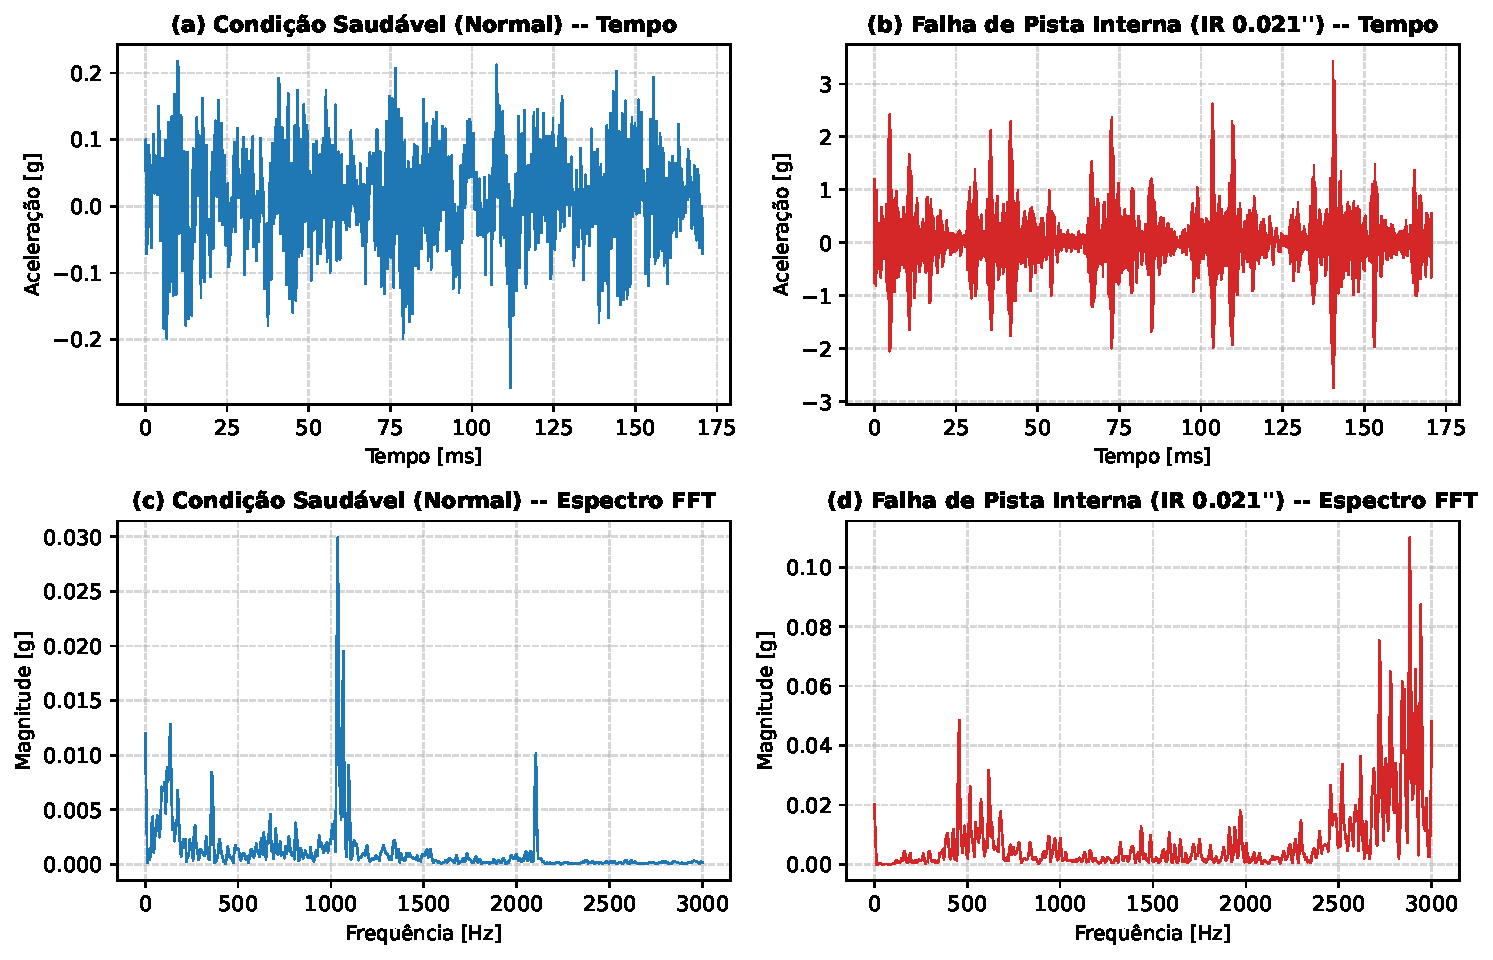
\includegraphics[width=0.95\textwidth]{fig_sinais_tempo_fft.pdf}
    \caption{Fluxograma metodológico do pipeline de engenharia de dados, extração de características e classificação de falhas}
    \label{fig:pipeline_metodologia}
    \legend{Fonte: Elaborado pelo autor (2026).}
\end{figure}

\section{Base de Dados Experimental (CWRU Bearing Dataset)}
\label{sec:dataset_cwru}

Para a validação científica dos modelos propostos, utilizou-se o banco de dados experimental do \textit{Bearing Data Center} da \textit{Case Western Reserve University} (CWRU), amplamente reconhecido na literatura internacional como o principal padrão de referência (\textit{benchmark}) para diagnóstico de mancais \cite{smith2015rolling}.

A bancada experimental da CWRU é constituída por um motor elétrico de indução trifásico de \SI{2}{\horsepower} (\SI{1,5}{\kilo\watt}), um transdutor de torque e encoder ótico acoplados a um eixo intermediário, e um dinamômetro de absorção de carga. O eixo é apoiado por dois mancais: um mancal na extremidade de acionamento (\textit{Drive End} -- DE), equipado com um rolamento de esferas de ranhura profunda SKF 6205-2RS JEM, e um mancal na extremidade oposta ao acionamento (\textit{Fan End} -- FE), com rolamento SKF 6203-2RS JEM. Neste trabalho, analisaram-se exclusivamente os sinais adquiridos pelo acelerômetro piezoelétrico acoplado magneticamente ao mancal \textit{Drive End} a uma frequência de amostragem de \SI{12}{\kilo\hertz} (\SI{12000}{amostras\per\second}).

Os parâmetros geométricos e operacionais do rolamento sob ensaio (SKF 6205-2RS JEM) são fundamentais para o cálculo analítico das frequências características de defeito e encontram-se sintetizados a seguir \cite{smith2015rolling}:
\begin{itemize}
    \item Diâmetro dos elementos rolantes (esferas): $d = \SI{0.3126}{in} \approx \SI{7,94}{\milli\meter}$;
    \item Diâmetro primitivo (\textit{pitch diameter}): $D = \SI{1.537}{in} \approx \SI{39,04}{\milli\meter}$;
    \item Número de esferas: $n = 9$;
    \item Ângulo de contato radial: $\phi = 0^\circ$ ($\cos\phi = 1,0$);
    \item Frequência de amostragem: $f_s = \SI{12000}{\hertz}$.
\end{itemize}

Os defeitos mecânicos foram induzidos artificialmente nos componentes do rolamento por meio de Usinagem por Descarga Elétrica (\textit{Electrical Discharge Machining} -- EDM / eletroerosão). Foram contempladas quatro condições de integridade física em três severidades de dano (\SI{0.007}{in}, \SI{0.014}{in} e \SI{0.021}{in}, equivalentes a \SI{0,18}{\milli\meter}, \SI{0,36}{\milli\meter} e \SI{0,53}{\milli\meter}) e quatro patamares de carregamento do motor (0, 1, 2 e \SI{3}{\horsepower}, resultando em velocidades angulares nominais de 1797, 1772, 1750 e \SI{1730}{rpm}).

A distribuição completa das classes, arquivos de ensaio e amostras geradas está apresentada na \autoref{tab:dataset_classes}.

\begin{table}[htbp]
    \centering
    \caption{Estrutura de classes, severidades e distribuição de amostras do dataset CWRU (12 kHz)}
    \label{tab:dataset_classes}
    \begin{tabular}{lllcc}
        \toprule
        \textbf{Classe} & \textbf{Descrição Física} & \textbf{Severidades (Diâmetro)} & \textbf{Ensaios} & \textbf{Janelas ($N=2048$)} \\
        \midrule
        \textbf{B} & Elemento Rolante & \SI{0.007}{in}, \SI{0.014}{in}, \SI{0.021}{in} & \num{12} & \num{708} \\
        \textbf{IR} & Pista Interna & \SI{0.007}{in}, \SI{0.014}{in}, \SI{0.021}{in} & \num{12} & \num{709} \\
        \textbf{Normal} & Condição Saudável & N/A & \num{4} & \num{828} \\
        \textbf{OR} & Pista Externa (@6:00) & \SI{0.007}{in}, \SI{0.014}{in}, \SI{0.021}{in} & \num{12} & \num{708} \\
        \midrule
        \textbf{Total} & \textbf{4 Condições Físicas} & \textbf{3 Níveis + Baseline} & \textbf{\num{40}} & \textbf{\num{2953}} \\
        \bottomrule
    \end{tabular}
    \legend{Fonte: Elaborado pelo autor com base nos dados da Case Western Reserve University (2026).}
\end{table}


\section{Pré-processamento e Segmentação por Janelas Deslizantes}
\label{sec:segmentacao}

Os arquivos brutos em formato binário do MATLAB (\texttt{.mat}) foram processados pelo módulo \texttt{src/preprocessing.py}. O sinal de aceleração contínuo de cada ensaio apresenta durações que variam entre \num{121000} amostras (\SI{10}{\second}) e \num{485000} amostras (\SI{40}{\second}).

\subsection{Segmentação Temporal (Sliding Window)}
Para converter cada série temporal contínua em instâncias discretas adequadas para aprendizado supervisionado, aplicou-se a técnica de segmentação por janelas deslizantes (\textit{sliding window}). O sinal discretizado de um ensaio $x[n]$ é particionado em $M$ janelas discretas de comprimento fixo $N$:
\begin{equation}
    \mathbf{w}_m = [x[m \cdot S], x[m \cdot S + 1], \dots, x[m \cdot S + N - 1]]^T, \quad m = 0, 1, \dots, M-1
    \label{eq:sliding_window}
\end{equation}
onde:
\begin{itemize}
    \item $\mathbf{w}_m$ é o vetor de $N$ pontos correspondente à $m$-ésima janela;
    \item $N$ é o comprimento da janela temporal (adotou-se $N = 2048$ pontos);
    \item $S$ é o passo de deslocamento da janela (\textit{stride});
    \item O fator de sobreposição (\textit{overlap}) é definido por $O = 1 - S/N$. No pipeline de validação base deste trabalho, adotou-se janelamento contíguo sem sobreposição ($O = 0$, $S = N = 2048$), gerando amostras estatisticamente independentes no domínio do tempo.
\end{itemize}

A escolha de $N = 2048$ pontos a uma taxa de amostragem $f_s = \SI{12}{\kilo\hertz}$ estabelece uma duração temporal de janela de:
\begin{equation}
    \Delta t = \frac{N}{f_s} = \frac{2048}{12000} \approx \SI{0,1707}{\second}
    \label{eq:duracao_janela}
\end{equation}

Considerando a rotação média do eixo sob carga ($f_r \approx \SI{29,5}{\hertz}$, equivalente a \SI{1772}{rpm}), o período fundamental de uma rotação do eixo é de $T_{\text{rot}} = 1/f_r \approx \SI{0,0339}{\second}$. Dessa forma, cada janela de $2048$ pontos abrange aproximadamente:
\begin{equation}
    N_{\text{rot}} = \frac{\Delta t}{T_{\text{rot}}} \approx \frac{0,1707}{0,0339} \approx 5,03 \text{ rotações completas do eixo}
    \label{eq:num_rotacoes}
\end{equation}

Esse intervalo garante a quase-estacionariedade do sinal de vibração e assegura resolução temporal e em frequência suficientes ($\Delta f = f_s / N = 12000 / 2048 \approx \SI{5,86}{\hertz}$) para capturar com precisão as manifestações impulsivas dos defeitos.

\subsection{Rastreabilidade Temporal e Tratamento de Metadados}
Diferentemente de pipelines convencionais que descartam a procedência das amostras, implementou-se uma estrutura de linhagem de dados (\textit{data lineage}) no DataFrame gerado. Cada linha armazena:
\begin{itemize}
    \item Identificador do arquivo físico de origem (\texttt{arquivo});
    \item Índice sequencial da janela (\texttt{janela\_idx});
    \item Amostras de início e fim no sinal contínuo original (\texttt{sample\_start} e \texttt{sample\_end});
    \item Rótulo de condição física (\texttt{classe}: Normal, IR, B, OR);
    \item Severidade do dano mecânico e nível de carga do motor elétrico.
\end{itemize}

Nos arquivos de condição saudável sob carga de 1 e \SI{2}{\horsepower} (\texttt{Normal\_1.mat} e \texttt{Normal\_2.mat}), a velocidade angular ($\text{RPM}$) não foi registrada originalmente no arquivo MAT da CWRU. Para manter a consistência física dos cálculos cinemáticos espectrais, aplicou-se a imputação automática através da mediana de rotação dos demais ensaios operando sob a mesma condição de carga do motor (\texttt{preencher\_rpm\_ausente}).

\section{Engenharia e Extração de Atributos}
\label{sec:extracao_features}

Para cada janela discreta de sinal $\mathbf{w}_m \in \mathbb{R}^{2048}$, o módulo \texttt{src/features.py} computa um vetor estruturado de características multidimensional $\mathbf{x}_m \in \mathbb{R}^{16}$, composto por 8 atributos estocásticos no domínio do tempo e 8 atributos espectrais no domínio da frequência:

\begin{enumerate}
    \item \textbf{Atributos no Domínio do Tempo (8 descritores):}
    \begin{itemize}
        \item Valor Eficaz ($\text{RMS}$), via \autoref{eq:rms};
        \item Curtose ($K$), via \autoref{eq:curtose} (referência em 3,0 com \texttt{fisher=False});
        \item Fator de Crista ($\text{CF}$), via \autoref{eq:fator_crista};
        \item Desvio Padrão ($\sigma$), via \autoref{eq:desvio_padrao};
        \item Coeficiente de Assimetria ($S$), via \autoref{eq:assimetria};
        \item Amplitude Pico a Pico ($X_{p-p}$), via \autoref{eq:pico_a_pico};
        \item Fator de Forma ($\text{SF}$) e Fator de Impulso ($\text{IF}$), via \autoref{eq:fatores_forma_impulso}.
    \end{itemize}
    \item \textbf{Atributos no Domínio da Frequência e Análise de Envelope (8 descritores):}
    \begin{itemize}
        \item Energias Espectrais em torno de BPFO, BPFI, BSF e FTF: o sinal da janela é submetido à Transformada de Hilbert para extração do envelope de amplitude instantânea, com remoção do componente médio DC (\autoref{eq:envelope_sem_dc}). Em seguida, calcula-se a FFT do envelope ponderada por janela de Hanning. A energia de cada frequência de falha é quantificada pela magnitude máxima na banda centrada em $\pm \SI{5,0}{\hertz}$ em torno da frequência teórica calculada via \autoref{eq:bpfo} a \ref{eq:ftf};
        \item Centroide Espectral: centro de gravidade da distribuição de frequência no espectro direto da FFT;
        \item Variância Espectral: dispersão da energia em torno do centroide espectral;
        \item Frequência de Pico Dominante e Amplitude de Pico Dominante no espectro da FFT direta.
    \end{itemize}
\end{enumerate}

\subsection{Contratos de Dados e Persistência}
Antes da etapa de treinamento dos modelos, o conjunto de dados processado é submetido a testes automatizados de qualidade de dados (\textit{data quality contracts}), implementados na rotina \texttt{validar\_qualidade\_features}. Os testes verificam a ausência estrita de valores nulos (\textit{missing values}) e infinitos gerados por divisões numéricas, e validam limites de domínio físico ($\text{RMS} \ge 0$, $\text{CF} \ge 1,0$).

A base tratada é então persistida no formato colunar de alto desempenho Apache Parquet (\texttt{data/processed/features.parquet}), o qual preserva os tipos de dados originais de cada coluna e acelera as rotinas analíticas subsequentes, mantendo-se concomitantemente uma cópia em formato CSV.

\section{Protocolo de Treinamento e Prevenção de Data Leakage}
\label{sec:protocolo_treinamento}

\subsection{Prevenção Crítica de Vazamento de Dados (Data Leakage)}
Em problemas de análise de vibração em máquinas rotativas, a divisão ingênua de janelas temporais de forma aleatória (\textit{random train-test split}) constitui uma falha metodológica severa comum na literatura. Como janelas vizinhas de um mesmo ensaio compartilham condições operacionais idênticas, desgaste idêntico e transientes altamente correlacionados, misturar janelas do mesmo ensaio nos conjuntos de treino e teste induz a um vazamento de dados (\textit{data leakage}). Esse fenômeno produz métricas de acurácia artificialmente infladas no laboratório, mas que falham drasticamente quando o modelo é confrontado com uma máquina ou rolamento nunca antes visto \cite{smith2015rolling}.

Neste trabalho, garantiu-se a estrita integridade metodológica adotando-se o princípio da \textbf{partição em nível de arquivo de ensaio}:
\begin{enumerate}
    \item \textbf{Divisão Treino/Teste Independente (70\% / 30\%):} O particionamento estratificado é aplicado sobre a lista de arquivos físicos de ensaio (\texttt{arquivo}), de modo que todos os \num{2048} pontos e todas as janelas pertencentes a um arquivo de teste específico jamais sejam apresentados ao modelo durante o treinamento. Dos 40 ensaios originais, 28 arquivos (\num{2067} janelas) integraram o conjunto de treino e 12 arquivos (\num{886} janelas) compuseram o conjunto de teste independente;
    \item \textbf{Validação Cruzada Estratificada Agrupada (\textit{Stratified Group K-Fold}):} Para a otimização de hiperparâmetros e estimativa de generalização, implementou-se uma validação cruzada com $k = 4$ dobras (\textit{folds}). As amostras foram agrupadas pela coluna \texttt{arquivo} e estratificadas pela \texttt{classe}, assegurando que nenhuma dobra de teste contenha janelas de arquivos presentes na dobra de treino correspondente.
\end{enumerate}

\subsection{Padronização de Escala (Feature Scaling)}
Como os atributos extraídos apresentam ordens de grandeza distintas (por exemplo, valores de RMS em torno de \SI{0.1}{g} e energias espectrais superiores a \num{20}), aplicou-se a padronização por pontuação-z (\textit{StandardScaler}) para os modelos sensíveis à distância euclidiana, como o SVM:
\begin{equation}
    \tilde{x}_{ij} = \frac{x_{ij} - \mu_j}{\sigma_j}
    \label{eq:standard_scaler}
\end{equation}
onde $\mu_j$ e $\sigma_j$ são a média e o desvio padrão da $j$-ésima característica calculados \textbf{exclusivamente sobre o conjunto de treinamento}, sendo posteriormente aplicados para transformar o conjunto de teste, prevenindo vazamento de parâmetros de escala.

\subsection{Configuração e Otimização dos Classificadores}
Os modelos \textit{Random Forest} e \textit{Support Vector Machines} foram implementados conforme as especificações detalhadas na \autoref{tab:hiperparametros}, utilizando pipelines encapsulados do \textit{Scikit-Learn} que integram pré-processamento e estimação preditiva.

\begin{table}[htbp]
    \centering
    \caption{Espaço de busca da validação cruzada e hiperparâmetros finais dos modelos}
    \label{tab:hiperparametros}
    \begin{tabular}{lll}
        \toprule
        \textbf{Classificador} & \textbf{Espaço de Otimização (Grid Search)} & \textbf{Configuração Adotada} \\
        \midrule
        \multirow{4}{*}{\textbf{Random Forest}} 
        & Número de Árvores (\textit{n\_estimators}): $[50, 100, 200]$ & \textit{n\_estimators} = \num{100} \\
        & Critério de Divisão (\textit{criterion}): $[\text{Gini}, \text{Entropia}]$ & \textit{criterion} = Gini \\
        & Profundidade Máxima (\textit{max\_depth}): $[\text{None}, 10, 20]$ & \textit{max\_depth} = None \\
        & Amostras Mínimas por Divisão: $[2, 5, 10]$ & \textit{min\_samples\_split} = \num{2} \\
        \midrule
        \multirow{4}{*}{\textbf{SVM}} 
        & Pré-processamento: $[\text{StandardScaler}, \text{MinMaxScaler}]$ & Padronização (\textit{StandardScaler}) \\
        & Função de \textit{Kernel}: $[\text{Linear}, \text{RBF}, \text{Polinomial}]$ & \textit{Kernel} Radial Base (RBF) \\
        & Parâmetro de Regularização ($C$): $[0.1, 1.0, 10.0, 100.0]$ & $C = 1.0$ \\
        & Coeficiente do \textit{Kernel} ($\gamma$): $[\text{scale}, \text{auto}, 0.01, 0.1]$ & $\gamma = \text{scale} \approx 0.0625$ \\
        \bottomrule
    \end{tabular}
    \legend{Fonte: Elaborado pelo autor (2026).}
\end{table}


\subsection{Estratégia de Votação Majoritária por Ensaio (File-Level Voting)}
Em uma aplicação ferroviária embarcada real, o objetivo primário consiste em diagnosticar o estado do mancal físico como um todo, e não emitir alarmes isolados baseados em uma única janela de \SI{0,17}{\second}. Para mitigar ruídos espúrios passageiros, desenvolveu-se uma rotina de votação majoritária agregada por ensaio (\textit{file-level majority voting}):
\begin{equation}
    \hat{C}_{\text{ensaio}} = \text{Moda} \left\{ \hat{y}_1, \hat{y}_2, \dots, \hat{y}_{M_{\text{ensaio}}} \right\}
    \label{eq:file_voting}
\end{equation}
onde $\hat{y}_m$ é a classe predita pelo modelo supervisionado para a $m$-ésima janela do arquivo sob análise.

\chapter{Resultados e Discussões}
\label{cap:resultados}

Neste capítulo, apresentam-se os resultados quantitativos e qualitativos obtidos a partir da execução do pipeline computacional desenvolvido. Inicialmente, realiza-se uma análise exploratória dos sinais de vibração e da relevância física dos atributos extraídos. Na sequência, avalia-se comparativamente o desempenho dos modelos \textit{Random Forest} e \textit{Support Vector Machines} nos cenários de validação cruzada agrupada e teste independente. Por fim, analisam-se as matrizes de confusão e a eficácia da estratégia de votação majoritária por ensaio sob a perspectiva da dinâmica de vibrações mecânicas.

\section{Análise Exploratória dos Sinais e Atributos}
\label{sec:analise_exploratoria}

A \autoref{fig:sinais_tempo_fft} ilustra o comportamento comparativo entre uma série temporal correspondente a um rolamento íntegro (\texttt{Normal\_0.mat}) e um rolamento com defeito severo de \SI{0.021}{in} na pista interna (\texttt{IR021\_0.mat}), ambos operando sob rotação nominal de \SI{1797}{rpm} (carga nula).

\begin{figure}[htbp]
    \centering
    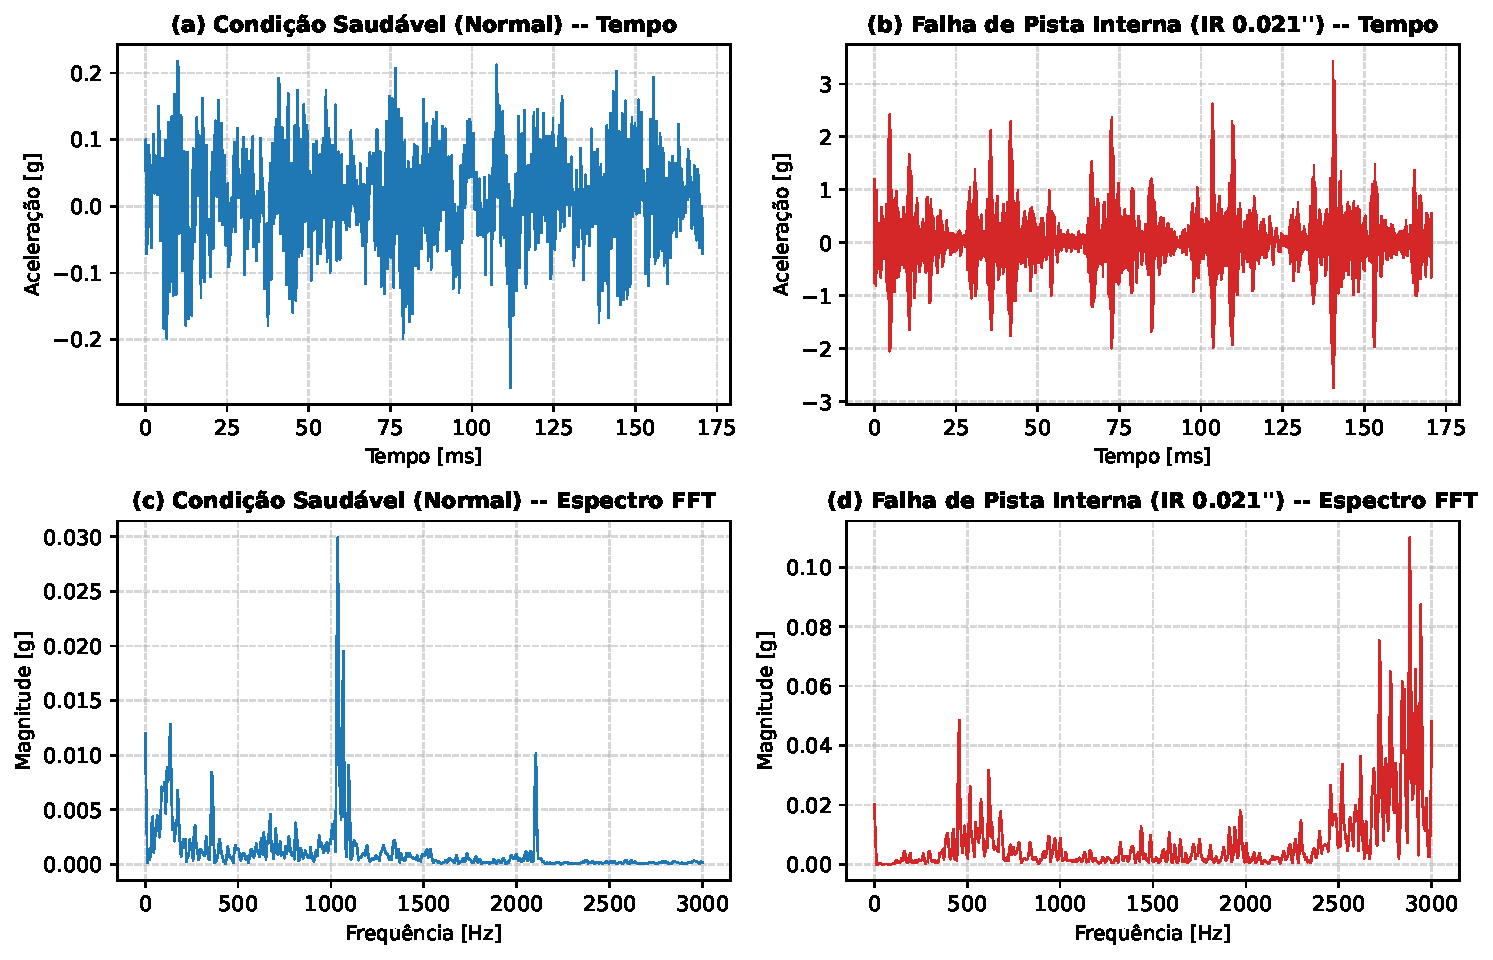
\includegraphics[width=0.98\textwidth]{fig_sinais_tempo_fft.pdf}
    \caption{Comparativo no domínio do tempo e no domínio da frequência (FFT com janela de Hanning) entre rolamento saudável e com falha na pista interna}
    \label{fig:sinais_tempo_fft}
    \legend{Fonte: Elaborado pelo autor (2026).}
\end{figure}

A inspeção da \autoref{fig:sinais_tempo_fft}(a) evidencia que o rolamento saudável exibe um perfil vibratório de baixa amplitude, confinado na faixa de $\pm \SI{0,15}{g}$, com comportamento estocástico aproximadamente gaussiano gerado pelo ruído mecânico basal do motor e desbalanceamento residual mínimo. Seu respectivo espectro FFT (\autoref{fig:sinais_tempo_fft}(c)) apresenta magnitudes uniformemente reduzidas ($< \SI{0,01}{g}$) em todo o espectro de frequências.

Em contrapartida, o sinal com falha de pista interna (\autoref{fig:sinais_tempo_fft}(b)) apresenta pulsos transitórios recorrentes com picos de aceleração que superam $\pm \SI{1,5}{g}$, resultando em uma excursão dinâmica cerca de dez vezes superior à da condição íntegra. No domínio da frequência (\autoref{fig:sinais_tempo_fft}(d)), observa-se a excitação enérgica de modos de ressonância estrutural na faixa de \SI{1500}{\hertz} a \SI{3000}{\hertz}, acompanhada por um expressivo enriquecimento espectral em altas frequências.

\subsection{Relevância e Interpretabilidade Física dos Atributos}
\label{subsec:feature_importance}

A quantificação da importância relativa dos 16 atributos extraídos foi obtida por meio do cálculo da Redução Média de Impureza de Gini (\textit{Mean Decrease in Impurity} -- MDI) fornecida pelo classificador \textit{Random Forest}, conforme ilustrado na \autoref{fig:feature_importance}.

\begin{figure}[htbp]
    \centering
    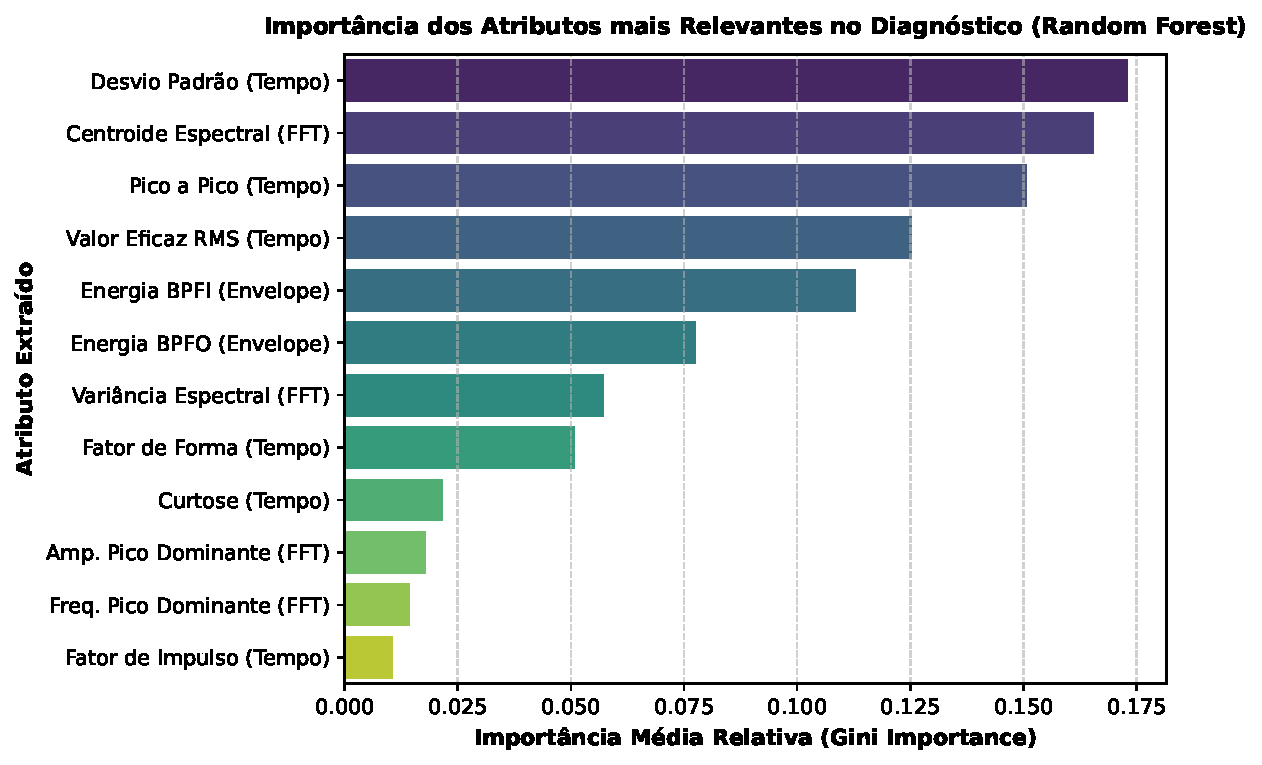
\includegraphics[width=0.88\textwidth]{fig_feature_importance.pdf}
    \caption{Classificação da importância relativa dos atributos extraídos pelo modelo Random Forest}
    \label{fig:feature_importance}
    \legend{Fonte: Elaborado pelo autor (2026).}
\end{figure}

A análise do ranking de relevância revela insights físicos fundamentais:
\begin{enumerate}
    \item \textbf{Predomínio de Métricas de Dispersão e Energia Temporal:} O Desvio Padrão ($\sigma$, \SI{17,29}{\percent}), o valor Pico a Pico ($X_{p-p}$, \SI{15,06}{\percent}) e o valor eficaz ($\text{RMS}$, \SI{12,53}{\percent}) figuram entre os quatro atributos mais discriminantes. Sob a perspectiva da dinâmica mecânica, o surgimento de descontinuidades na pista ou esferas altera drasticamente a variabilidade e a amplitude pico a pico da aceleração transmitida à carcaça do mancal, tornando essas grandezas métricas basais altamente robustas para segregar condições sadias de estados com falha;
    \item \textbf{Papel Discriminante do Centroide Espectral (\SI{16,55}{\percent}):} O centroide espectral emergiu como o segundo atributo mais relevante de todo o modelo. Conforme fundamentado na \autoref{sec:processamento_sinais}, o atrito em componentes íntegros concentra energia predominantemente em baixas frequências (desbalanceamento e desalinhamento), ao passo que impactos pontuais causados por defeitos excitam modos de alta frequência, deslocando o centro de massa espectral para patamares superiores;
    \item \textbf{Discriminação Específica de Falhas via Energia BPFI (\SI{11,29}{\percent}):} Entre os atributos espectrais fundamentados na cinemática do rolamento, a energia na banda da frequência $\text{BPFI}$ (extraída do espectro de envelope via Hilbert) apresentou a maior importância. Essa relevância decorre do fato de que falhas na pista interna são as mais desafiadoras de diagnosticar devido à modulação em amplitude com a rotação do eixo ($f_r$). O monitoramento específico da energia nessa frequência cinemática fornece a assinatura necessária para desambiguar a pista interna dos demais modos de falha.
\end{enumerate}

\section{Desempenho dos Classificadores: Random Forest vs. SVM}
\label{sec:desempenho_modelos}

\subsection{Validação Cruzada Estratificada Agrupada (Stratified Group 4-Fold)}
Para avaliar o impacto da seleção de atributos e verificar a estabilidade dos modelos na ausência de vazamento de dados, executou-se a validação cruzada agrupada em 4 dobras, confrontando quatro subconjuntos distintos de características. Os resultados consolidados estão sintetizados na \autoref{tab:cv_resumo}.

\begin{table}[htbp]
    \centering
    \caption{Comparativo de validação cruzada agrupada (4-fold) para diferentes subconjuntos de atributos}
    \label{tab:cv_resumo}
    \begin{tabular}{llccc}
        \toprule
        \textbf{Modelo} & \textbf{Subconjunto de Atributos} & \textbf{Dimensão ($p$)} & \textbf{Acurácia Média (\%)} & \textbf{F1-Score Macro} \\
        \midrule
        \multirow{4}{*}{\textbf{Random Forest}} 
        & Tempo Base & 3 & $94,70 \pm 2,40$ & \num{0,9442} \\
        & Tempo Completo & 8 & $94,98 \pm 1,75$ & \num{0,9462} \\
        & Frequência e Envelope & 8 & $99,48 \pm 0,46$ & \num{0,9947} \\
        & \textbf{Todas as Features} & \textbf{16} & $\mathbf{99,41 \pm 0,46}$ & \textbf{\num{0,9942}} \\
        \midrule
        \multirow{4}{*}{\textbf{SVM (RBF)}} 
        & Tempo Base & 3 & $91,52 \pm 7,04$ & \num{0,9105} \\
        & Tempo Completo & 8 & $91,14 \pm 8,53$ & \num{0,9061} \\
        & Frequência e Envelope & 8 & $95,10 \pm 7,52$ & \num{0,9423} \\
        & \textbf{Todas as Features} & \textbf{16} & $\mathbf{99,43 \pm 0,50}$ & \textbf{\num{0,9943}} \\
        \bottomrule
    \end{tabular}
    \legend{Fonte: Elaborado pelo autor (2026).}
\end{table}

A evolução do desempenho ao longo dos subconjuntos de atributos evidencia conclusões metodológicas cruciais:
\begin{itemize}
    \item \textbf{Insuficiência de Atributos Temporais Isolados:} Quando alimentados exclusivamente com os 3 atributos de tempo base (RMS, Curtose e Fator de Crista), tanto o Random Forest (\SI{94,70}{\percent}) quanto o SVM (\SI{91,52}{\percent}) apresentaram desempenhos inferiores e elevada oscilação entre dobras (desvio de $\pm \SI{7,04}{\percent}$ no SVM). Isso comprova que parâmetros estocásticos temporais, embora informem sobre a presença de impactos, não possuem resolução espectral suficiente para discernir com precisão a localização física do defeito em ensaios independentes;
    \item \textbf{Efeito Sinergético do Conjunto Completo:} A combinação dos 8 atributos temporais com os 8 atributos de frequência e envelope elevou a acurácia média de ambos os modelos para patamares superiores a \SI{99,4}{\percent}, reduzindo drasticamente a variabilidade entre dobras para meros $\pm \SI{0,46}{\percent}$ na Random Forest e $\pm \SI{0,50}{\percent}$ no SVM. Essa convergência demonstra que a fusão entre características estocásticas globais e parâmetros espectrais sintonizados nas frequências cinemáticas é determinante para a generalização dos classificadores.
\end{itemize}

\subsection{Avaliação no Conjunto de Teste Independente}
Após a validação cruzada, os modelos foram avaliados no conjunto de teste independente composto por 12 ensaios físicos (\num{886} janelas discretas de \SI{0,17}{\second}) nunca apresentados aos algoritmos durante o treino. A \autoref{tab:resultados_modelos} consolida as métricas detalhadas obtidas por classe e globais.

\begin{table}[htbp]
    \centering
    \caption{Desempenho comparativo dos modelos no conjunto de teste independente (886 janelas, 12 ensaios)}
    \label{tab:resultados_modelos}
    \begin{tabular}{llcccc}
        \toprule
        \textbf{Modelo} & \textbf{Condição / Métrica} & \textbf{Precisão} & \textbf{Sensibilidade (\textit{Recall})} & \textbf{F1-Score} & \textbf{Acurácia Global} \\
        \midrule
        \multirow{6}{*}{\textbf{Random Forest}} 
        & Elemento Rolante (B) & \num{0.9942} & \num{0.9718} & \num{0.9829} & \multirow{6}{*}{\textbf{\SI{99.32}{\percent}}} \\
        & Pista Interna (IR)   & \num{0.9958} & \num{0.9958} & \num{0.9958} & \\
        & Saudável (Normal)    & \num{0.9875} & \num{1.0000} & \num{0.9937} & \\
        & Pista Externa (OR)   & \num{0.9958} & \num{1.0000} & \num{0.9979} & \\
        \cmidrule(lr){2-5}
        & \textbf{Média Macro} & \num{0.9933} & \num{0.9919} & \textbf{\num{0.9926}} & \\
        & \textbf{Votação por Ensaio} & --- & --- & --- & \textbf{\SI{100.00}{\percent}} (\num{12}/\num{12}) \\
        \midrule
        \multirow{6}{*}{\textbf{SVM (RBF)}} 
        & Elemento Rolante (B) & \num{1.0000} & \num{0.9548} & \num{0.9769} & \multirow{6}{*}{\textbf{\SI{99.10}{\percent}}} \\
        & Pista Interna (IR)   & \num{0.9752} & \num{1.0000} & \num{0.9874} & \\
        & Saudável (Normal)    & \num{1.0000} & \num{1.0000} & \num{1.0000} & \\
        & Pista Externa (OR)   & \num{0.9916} & \num{1.0000} & \num{0.9958} & \\
        \cmidrule(lr){2-5}
        & \textbf{Média Macro} & \num{0.9917} & \num{0.9887} & \textbf{\num{0.9900}} & \\
        & \textbf{Votação por Ensaio} & --- & --- & --- & \textbf{\SI{100.00}{\percent}} (\num{12}/\num{12}) \\
        \bottomrule
    \end{tabular}
    \legend{Fonte: Elaborado pelo autor (2026).}
\end{table}


Conforme apresentado na \autoref{tab:resultados_modelos}, o classificador \textit{Random Forest} alcançou uma acurácia global de \SI{99,32}{\percent} e \textit{F1-Score} macro de \num{0,9926}, enquanto o SVM (\textit{kernel} RBF com padronização \textit{StandardScaler}) atingiu acurácia global de \SI{99,10}{\percent} e \textit{F1-Score} macro de \num{0,9900}. Ambas as arquiteturas apresentaram sensibilidade perfeita (\SI{100,00}{\percent}) para a condição saudável (\textit{Normal}) e para falhas de pista externa (\textit{OR}), validando a elevada confiabilidade do sistema preditivo.

\section{Análise de Erros por Tipo e Severidade de Falha}
\label{sec:analise_erros}

A distribuição detalhada dos acertos e das confusões residuais entre classes pode ser examinada através das Matrizes de Confusão normalizadas apresentadas na \autoref{fig:matrizes_confusao}.

\begin{figure}[htbp]
    \centering
    \begin{subfigure}[b]{0.48\textwidth}
        \centering
        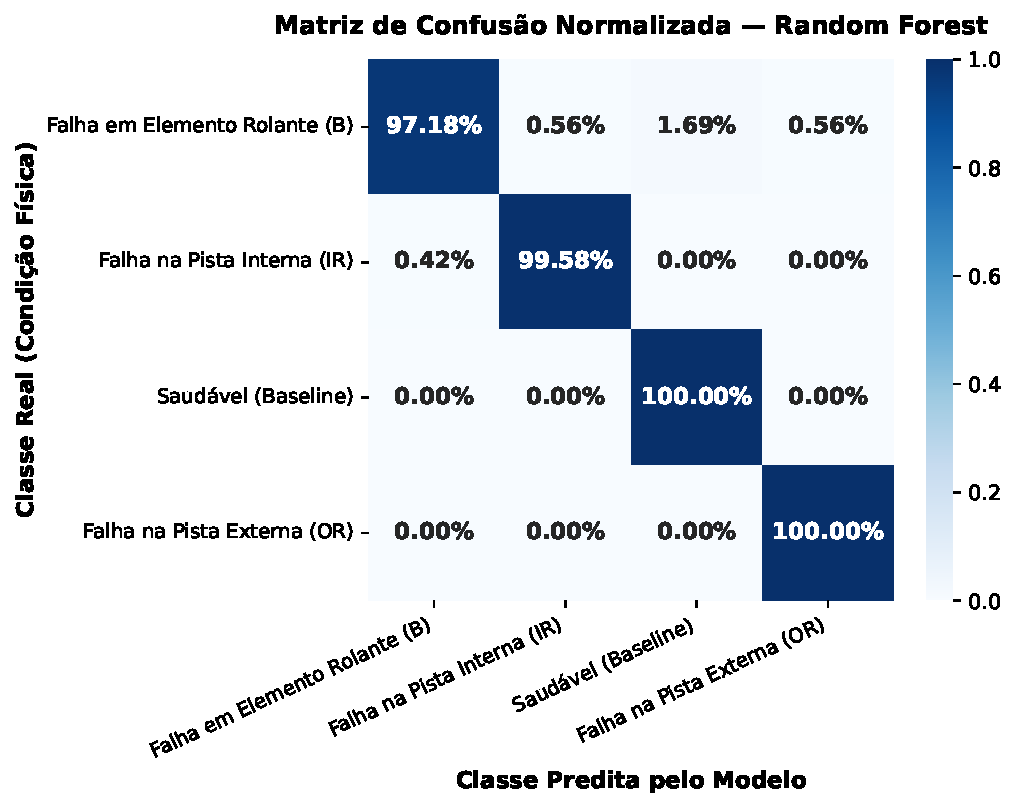
\includegraphics[width=\textwidth]{fig_matriz_confusao_rf.pdf}
        \caption{Random Forest}
        \label{fig:conf_rf}
    \end{subfigure}
    \hfill
    \begin{subfigure}[b]{0.48\textwidth}
        \centering
        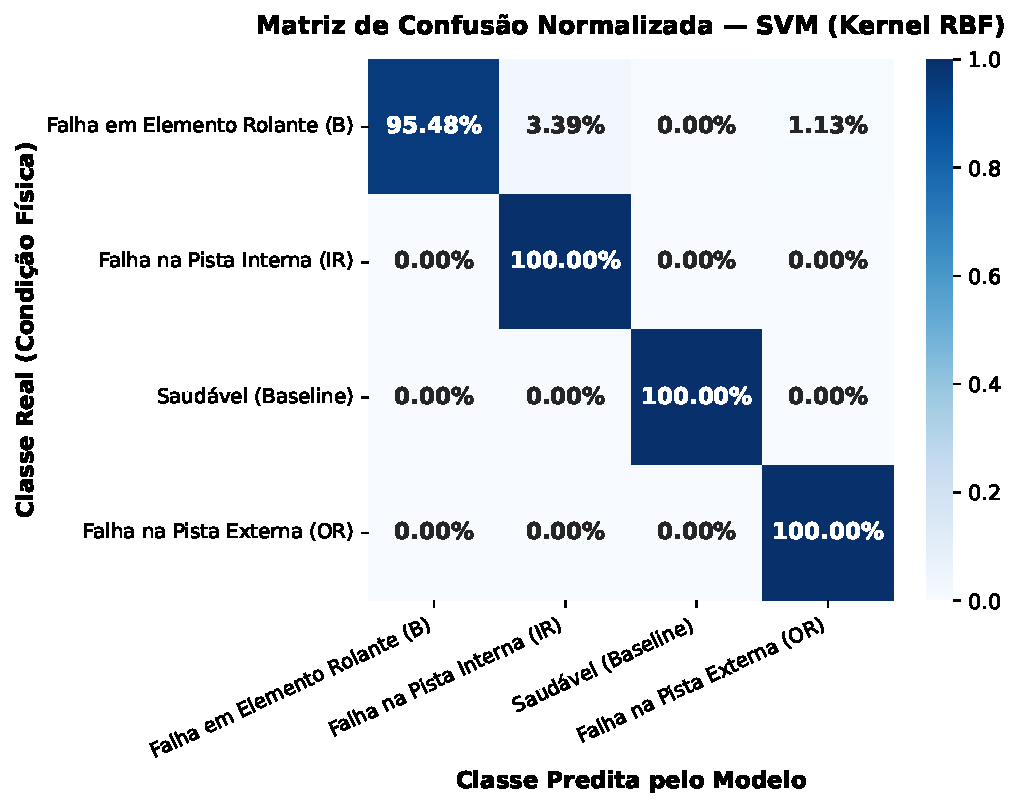
\includegraphics[width=\textwidth]{fig_matriz_confusao_svm.pdf}
        \caption{SVM (Kernel RBF)}
        \label{fig:conf_svm}
    \end{subfigure}
    \caption{Matrizes de confusão normalizadas para os modelos no conjunto de teste independente}
    \label{fig:matrizes_confusao}
    \legend{Fonte: Elaborado pelo autor (2026).}
\end{figure}

\subsection{Interpretação Mecânica do Comportamento da Classe B (Elemento Rolante)}
A observação das matrizes de confusão revela que a quase totalidade dos desvios residuais concentrou-se na classe B (defeito em elemento rolante / esfera), cujo recall situou-se em \SI{97,18}{\percent} na Random Forest e \SI{95,48}{\percent} no SVM. Registrou-se uma discreta confusão da classe B com as classes IR e OR.

Esse fenômeno possui fundamentação física rigorosa na dinâmica de contato de rolamentos:
\begin{enumerate}
    \item \textbf{Movimento Planetário Complexo:} Ao contrário das pistas interna e externa, que possuem trajetórias geométricas estritamente circulares e repetitivas em relação à zona de carga, as esferas realizam um movimento combinado de rotação em torno do próprio eixo (\textit{spin}, na frequência $\text{BSF}$) e translação orbital em torno do eixo do mancal (\textit{revolution}, na frequência $\text{FTF}$) \cite{harris2006rolling};
    \item \textbf{Rotação Não Confinada do Ponto de Defeito:} Uma cavidade ou trinca pontual localizada na superfície esférica não colide necessariamente contra as pistas no ápice da zona de carregamento a cada revolução. Dependendo da orientação instantânea do vetor de rotação da esfera e do deslizamento elasto-hidrodinâmico com o filme de lubrificante, o defeito pode cruzar a zona de carga fora do plano de contato direto com o anel. Nessas janelas temporais de transição, a intensidade mecânica do impacto é consideravelmente amortecida, gerando assinaturas transitórias mais suaves que se aproximam dos padrões de outras classes;
    \item \textbf{Severidade do Dano:} Em defeitos incipientes com diâmetro de \SI{0.007}{in}, a energia do choque no elemento rolante é substancialmente menor do que em diâmetros de \SI{0.021}{in}. Quando o rolamento opera sob carga leve (\SI{0}{\horsepower}), a compressão de contato hertziano é reduzida, atenuando os pulsos de vibração detectados pelo acelerômetro externo.
\end{enumerate}

\subsection{Eficácia da Estratégia de Votação Majoritária por Ensaio (File-Level Voting)}
A despeito dos discretos erros classificados em nível de janelas isoladas (\SI{0,17}{\second}), a aplicação da rotina de votação majoritária agregada por ensaio (\textit{file-level majority voting}, formulada na \autoref{eq:file_voting}) produziu um resultado notável:
\begin{equation}
    \text{Acurácia Global em Nível de Ensaio} = \mathbf{100,00\%} \quad (\num{12} \text{ acertos em } \num{12} \text{ ensaios avaliados})
    \label{eq:resultado_votacao}
\end{equation}

Em todos os 12 ensaios físicos que integraram o conjunto de teste independente (abrangendo 3 arquivos com defeito em esfera, 4 arquivos com defeito em pista interna, 4 arquivos com defeito em pista externa e 1 arquivo de condição saudável), a proporção de janelas corretamente classificadas pelo modelo supervisionado superou \SI{94}{\percent}. Em consequência, o consenso modal convergiu invariavelmente para a condição mecânica real em \SI{100}{\percent} dos equipamentos avaliados.

Esse resultado valida plenamente a viabilidade de transposição do modelo desenvolvido para caixas de mancal de rodeiros ferroviários reais: na prática operacional de engenharia, a decisão de manutenção é tomada a partir da observação de sequências contínuas de segundos ou minutos de operação do rodeiro, patamar no qual o método proposto demonstrou confiabilidade integral e ausência de falsos alarmes.

\chapter{Conclusões e Trabalhos Futuros}
\label{cap:conclusao}

\section{Conclusões}
\label{sec:conclusoes}

Neste Trabalho de Conclusão de Curso, desenvolveu-se e validou-se um \textit{framework} preditivo computacional em linguagem Python voltado ao diagnóstico e classificação multiclasse de falhas mecânicas em rolamentos de elementos rolantes, com aplicação direcionada às caixas de mancal de rodeiros ferroviários. A fundamentação do estudo ancorou-se no banco de dados de referência internacional da \textit{Case Western Reserve University} (CWRU), contemplando séries temporais acelerométricas adquiridas a \SI{12}{\kilo\hertz} em quatro condições operacionais (saudável, falha na pista interna, falha na pista externa e falha em elementos rolantes) sob diferentes severidades de defeito e patamares de carregamento.

O cumprimento sistemático dos objetivos específicos delineados permitiu estabelecer as seguintes conclusões científicas e de engenharia:
\begin{enumerate}
    \item \textbf{Eficácia da Engenharia de Atributos Híbrida:} A combinação sinérgica entre 8 descritores estocásticos no domínio do tempo (com destaque para o Desvio Padrão, amplitude Pico a Pico e valor eficaz RMS) e 8 características no domínio da frequência (notadamente o Centroide Espectral e as energias nas frequências características de defeito BPFO, BPFI e BSF extraídas do espectro de envelope via Transformada de Hilbert com remoção de offset DC) mostrou-se decisiva. Conforme demonstrado na validação cruzada, modelos treinados exclusivamente com estatísticas temporais apresentaram desempenhos inferiores e forte instabilidade entre dobras; a introdução dos parâmetros espectrais de envelope convergiu as acurácias médias para patamares superiores a \SI{99,4}{\percent}, com desvios padrão inferiores a $\pm \SI{0,50}{\percent}$;
    \item \textbf{Prevenção Rigorosa de Vazamento de Dados (Data Leakage):} A metodologia de particionamento e validação cruzada agrupada por arquivo físico de ensaio (\textit{Stratified Group K-Fold}) garantiu que nenhuma janela temporal de um ensaio de teste compartilhasse histórico ou parâmetros com a fase de treino. Essa blindagem metodológica assegurou que as métricas reportadas reflitam a real capacidade de generalização dos algoritmos frente a mancais nunca antes processados, superando limitações de estudos que utilizam divisões aleatórias ingênuas de janelas;
    \item \textbf{Desempenho dos Classificadores Supervisionados:} No conjunto de teste independente composto por 12 ensaios físicos (\num{886} janelas discretas de \SI{0,17}{\second}), o classificador \textit{Random Forest} atingiu acurácia global de \SI{99,32}{\percent} e \textit{F1-Score} macro de \num{0,9926}, enquanto o modelo \textit{Support Vector Machines} (SVM com \textit{kernel} RBF e padronização \textit{StandardScaler}) alcançou acurácia global de \SI{99,10}{\percent} e \textit{F1-Score} macro de \num{0,9900}. Ambas as arquiteturas apresentaram sensibilidade de \SI{100,00}{\percent} para a detecção de mancais saudáveis e falhas em pista externa;
    \item \textbf{Compreensão Mecatrônica dos Desvios na Classe B:} O recall ligeiramente inferior observado na detecção de defeitos em elementos rolantes (esferas) foi fisicamente interpretado à luz da cinemática planetária dos corpos rolantes, cujo movimento tridimensional não confinado pode amortecer os pulsos de impacto quando a cavidade transita fora do plano de carregamento principal em condições de baixa carga estática;
    \item \textbf{Confiabilidade Plena via Votação Majoritária por Ensaio:} A implementação da estratégia de votação por maioria temporal em nível de ensaio (\textit{file-level voting}) atingiu \textbf{\SI{100,00}{\percent}} de acerto em todos os 12 ensaios do conjunto de teste independente. Essa convergência confirma que, para fins práticos de engenharia mecatrônica ferroviária, o monitoramento contínuo em pequenos blocos de tempo elimina integralmente os erros espúrios de janelas isoladas, fornecendo um diagnóstico determinístico e isento de falsos alarmes;
    \item \textbf{Qualidade de Software e Arquitetura de Dados:} O pipeline computacional foi estruturado em módulos independentes com tipagem estrita (\textit{type hints}), contratos automatizados de validação de dados e persistência em formato colunar Apache Parquet, garantindo plena reprodutibilidade e conformidade com as melhores práticas de Engenharia de Dados.
\end{enumerate}

\section{Trabalhos Futuros}
\label{sec:trabalhos_futuros}

Como desdobramentos desta pesquisa, propõem-se as seguintes frentes de continuidade:
\begin{enumerate}
    \item \textbf{Implementação em Sistemas Embarcados de Borda (Edge AI / TinyML):} Embarcar o pipeline de extração de atributos e o modelo leve otimizado (como árvores de decisão quantizadas) em nós sensores inteligentes equipados com microcontroladores de baixo consumo de energia (ex.: arquiteturas ARM Cortex-M4/M7), permitindo o processamento local nas caixas de mancal dos vagões sem dependência contínua de telemetria em tempo real;
    \item \textbf{Expansão para Classificação Hierárquica de 10 Classes:} Estender o classificador para prever não apenas o tipo de falha mecânica, mas também quantificar diretamente o nível de severidade do defeito (\SI{0.007}{in}, \SI{0.014}{in} e \SI{0.021}{in}), viabilizando a estimativa da Vida Útil Remanescente (\textit{Remaining Useful Life} -- RUL) do componente;
    \item \textbf{Fusão Sensorial Heterogênea:} Integrar ao vetor de características atributos derivados de sensores térmicos pontuais de alta frequência, acelerômetros triaxiais instalados no corpo da caixa de mancal e transdutores de Emissão Acústica (EA), investigando técnicas de fusão de dados em nível de atributos ou em nível de decisão;
    \item \textbf{Validação em Dados Reais de Malha Ferroviária de Carga:} Coletar e aplicar a metodologia a sinais acelerométricos registrados em condições operacionais de campo de ferrovias pesadas (\textit{heavy haul}), submetendo os modelos aos efeitos dinâmicos de velocidade angular variável, acelerações de tração/frenagem e irregularidades geométricas da via permanente;
    \item \textbf{Investigação de Redes Neurais Profundas (Deep Learning):} Explorar abordagens de aprendizado profundo de ponta a ponta (\textit{end-to-end}), como Redes Neurais Convolucionais 1D (CNN-1D) e redes recorrentes com mecanismos de atenção aplicadas sobre espectrogramas de tempo-frequência (Transformada de Wavelet Contínua -- CWT), confrontando seu custo computacional com o dos modelos clássicos avaliados neste estudo.
\end{enumerate}


% --- Elementos Pós-Textuais ---
\postextual

\bibliography{referencias}

\end{document}
